\chapter{Cahier des charges}\label{ch:cahier}

L'année dernière, la société constatait sur ses solutions une véritable disparité de méthodologies d'intégration pour les documents. Chaque fonctionnalité intégrait les documents de manière différente, ce qui les amenait à constater qu'il était alors compliqué de répondre rapidement à ce type de besoins.

De plus, ils avaient d'une part les demandes d'import de nouveaux fournisseurs de carburant, mais également d'autre part la création du poste de CSM (Customer Success Manager), et enfin, à travers un besoin exprimé par l'un de ses grands clients, de plus en plus de besoins pour intégrer rapidement et efficacement de nouvelles typologies de documents.

Basé sur ce constat, ils ont donc défini qu'il était nécessaire de construire un outil permettant de répondre à ces besoins : le Pipeline documentaire.

Leur projet était qu'à terme, cet outil leur permettrait de généraliser l'intégration des fichiers dans leur solution. Il serait donc le point d'entrée central de tous les documents entrant dans chacun de leurs logiciels. L'ajout d'une nouvelle typologie de document serait simple et se ferait, pour la partie intégration du moins, au maximum à travers du paramétrage.

La section suivante montre comment le propriétaire du produit a exprimé les besoins concernant le Pipeline documentaire.

\section{Expression des besoins}

\subsection{Concepts généraux}

Dans sa conception, ce nouvel outil devra être le plus détaché possible du reste de l'ensemble applicatif, afin d'ensuite être mis à disposition et utilisé par l'ensemble de nos soft, de manière simple et intégré. Dans cet optique, l'outil devra donc être pensé pour être notre première ``Machine'', concept abordé lors de notre étude de la refonte global, qui est donc un outil logiciel à disposition de l'ensemble des autres applications, mais complètement autonome.

\subsection{Composition de l'outil}

\subsubsection{Déclencheurs}

Le concept de déclencheur devra être une partie spécifique de la conception de l'outil, répondant toujours aux même règles et permettant de lancer une intégration. Lorsqu'un déclencheur est ``appelé'' il lancera l'ensemble de l'intégration. Celui-ci fournira au guide toutes les informations nécessaire ainsi que le ou les fichiers à intégrer. Cependant, chaque déclencheur sera indépendant et répondra à une intégration spécifique. Un certain nombre de déclencheurs ont été identifiés dans le schéma architectural,Figure~\ref{fig:architectural-schema} cependant, cette liste n'est pas exhaustive.

\subsubsection{Guide}

Le guide sera, dans notre outil, le point central de l'intégration. Son but sera de charger la configuration adéquat afin de réaliser l'intégration, puis de faire passer le ou les fichiers à travers la chaîne d'intégration, en fonction de la configuration préalablement mise en œuvre. Finalement, le guide aura pour objectif de piloter l'ensemble de l'intégration du fichier, c'est à dire son bon passage ``à travers'' la chaine d'intégration.


\subsubsection{Configurations}

Les fichiers de configurations devront être réalisés pour déclarer tous nouvel import. Le fichier de configuration aura un format informatique, mais lisible par un développeur (json, yml \dots). Ces fichiers de configurations permettront, pour chaque type d'import, de déclarer les spécificités de celui-ci et d'ainsi déterminer chaque étape de l'import. Les principales informations présentes dans ces fichiers seront donc :

\begin{itemize}
    \item Le mapping des données
    \item Les détails du fichiers (encodage, extension \dots)
    \item Le type (csv, xml, pdf \dots)
    \item Le détail de la chaine d'intégration (classes à utiliser, OCR à réaliser \dots)
    \item Les traitements spécifiques à apporter au fichier (classe de lecture spécifique, classe de mapping spécifique \dots)
    \item \dots
\end{itemize}

\subsubsection{Chaine d'intégration}

Le guide aura pour but de déterminer, en se basant sur les informations du déclencheur et sur la configuration chargé, l'ensembles des maillons constituant la chaine d'intégration. Celle-ci sera composée d'étapes distinctes et unitaires, permettant d'arriver à l'intégration complète du fichier. Le guide se s'assurera que le ou les fichiers passent bien à travers chaque maillon de la chaine d'intégration.

\subsubsection{Actions transverses}

Les actions transverses devront être automatiques et aucune configuration ou code ne devra être intégré dans les parties spécifique d'un import. Cela signifie que le Pipeline documentaire en lui même devra les traiter, par défaut et sans action du développeur qui ajoutera une nouvelle chaine, un nouveau déclencheur ou une nouvelle configuration.

Les actions transverses seront :

\begin{itemize}
    \item \textbf{Documentation automatique :} les configurations sont automatiquement analysées et généreront une documentation exploitable simplement par un opérateur (extérieur à la R\&D comme support, commerce \dots)
    \item \textbf{Dashboard :} un ensemble de tableau devront rendre compte du bon fonctionnement du pipeline à chaque instant, ainsi qu'un récap des intégrations récentes.
    \item \textbf{Sauvegardes sérialisés :} l'ensemble des étapes devront être sauvegardés et sérialisés à des fins d'analyses. Cet historique pourra être purgé régulièrement, cependant, il parait interessant de conserver le fichier d'entrée et sa configuration attaché plus longtemps que la sérialisation des étapes.
\end{itemize}

\begin{figure}[ht]
    \centering
    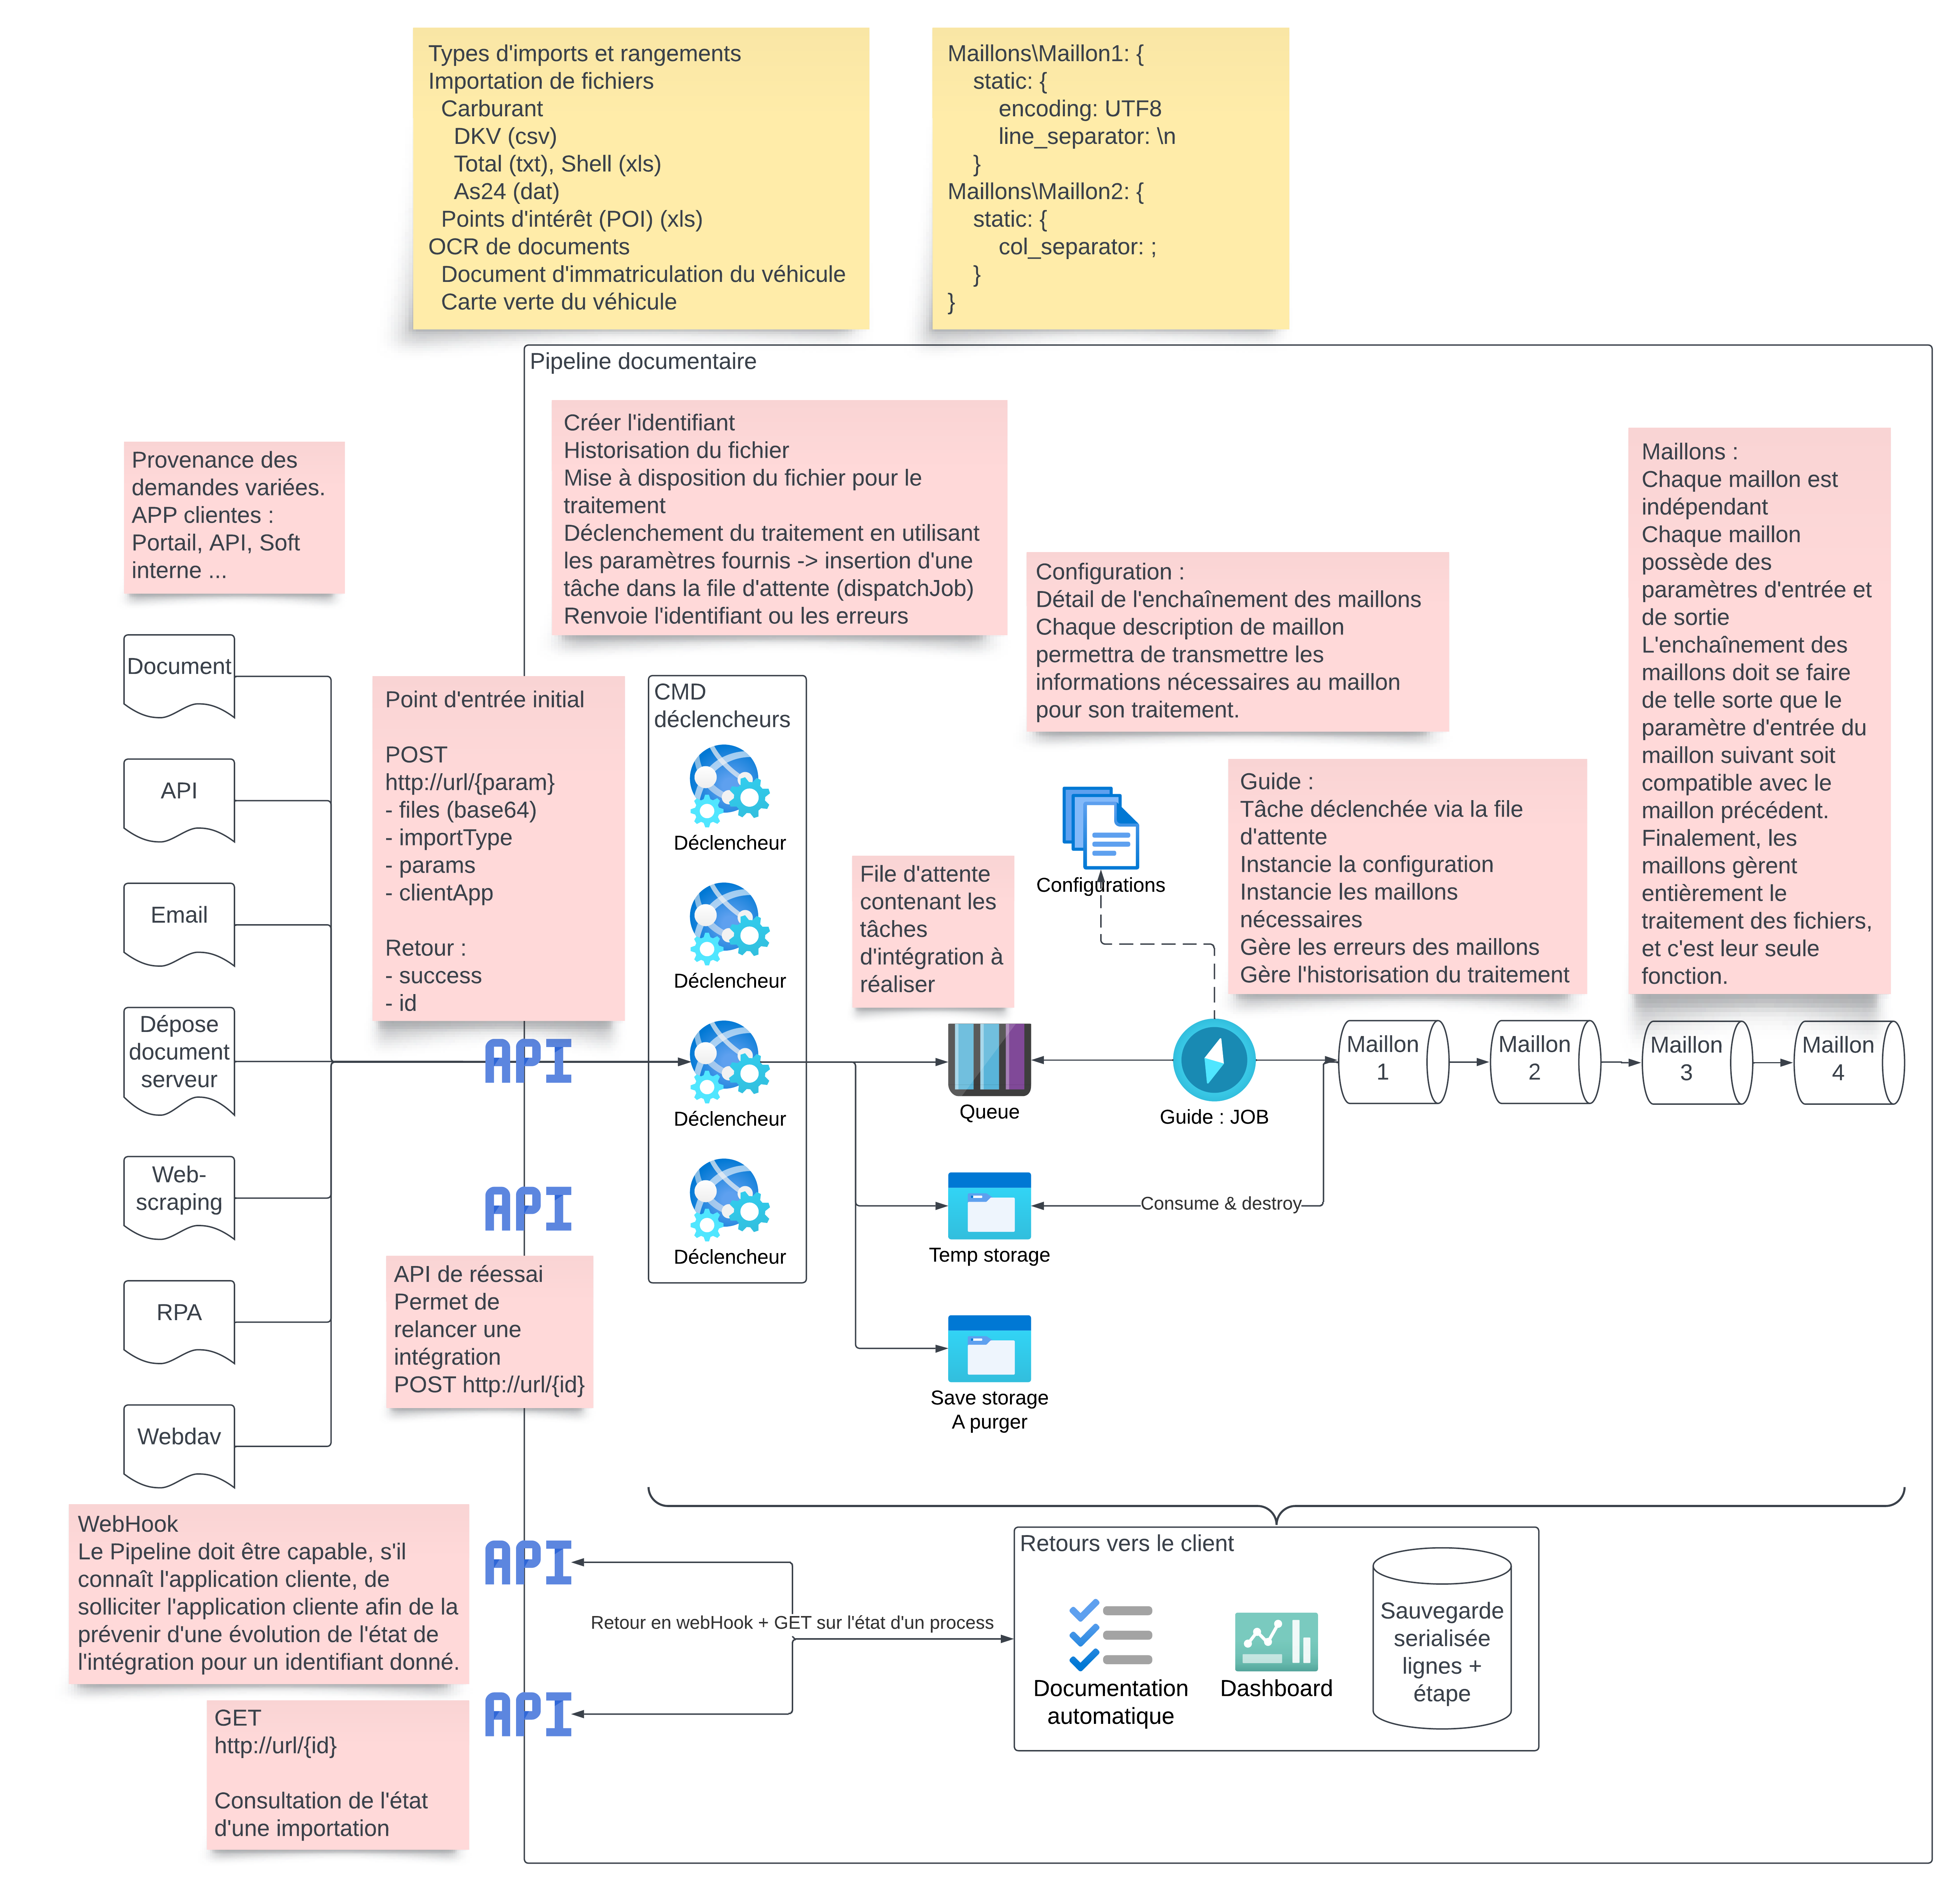
\includegraphics[width=\textwidth]{img/schema-architectural}
    \caption{Schéma architectural de Pipeline documentaire.}
    \label{fig:architectural-schema}
\end{figure}